\documentclass[11pt]{beamer}
% Packages
\usepackage{beamer-german}

% Title etc.
\title{Politisches Vertrauen}
\subtitle{Analyse politischer Unterstützung in der quantitativen Forschungspraxis}
\date{26. November 2021}
\author{B. Philipp Kleer}
\institute{Institut für Politikwissenschaft | Justus-Liebig-Universität Gießen}

\setbeamerfont{itemize/enumerate body}{size = \small}
\setbeamerfont{itemize/enumerate subbody}{size = \footnotesize}
\setbeamerfont{itemize/enumerate subsubbody}{size = \scriptsize}

% Datumspaket
\usepackage[german]{isodate}

% Table packages
\usepackage{booktabs}
\usepackage{longtable}

% bibtex-file
\usepackage[backend=biber]{biblatex}
\addbibresource{lit-s5.bib} 

\begin{document}

\begin{frame}
\titlepage
\end{frame}

%\begin{frame}[t]{Zusammenarbeit in der Pandemie}
%Wenn ihr in Gruppen arbeiten möchtet (Präsentation oder Hausarbeit), empfiehlt es sich Kollaborationsplattformen (z.B. Notion, Trello) oder Aufgabenmanager (z.B. Todoist). Über \shine{GitHub} funktioniert Dateienaustausch sehr gut (mehr dazu im Dezember), für Kommunikation ist es aber nicht geeignet. Alternativ kann ich euch auch in ILIAS eine Gruppe erstellen, in der ihr mit den Tools von \shine{ILIAS} zusammen arbeiten könnt (z.B. Etherpad, Blog, Wiki, Forum etc.).
%
%\end{frame}

\begin{frame}[t]{Political Trust}
\setbeamerfont{itemize/enumerate body}{size = \footnotesize}
\begin{itemize}
	\item „(…) we trust when we think the interests of those whom we trust are aligned in the right way with ours or when we think they are motivated to support our interest.“ \parencite[447]{Festenstein2019} \pause
	\item A trust B with respect to X \parencite[449]{Festenstein2019} \pause
	\item felt betrayal is more than disappointed expectations \parencite[450]{Festenstein2019} \pause
	\item Also moral norm of honesty disregarded \pause
	\item Position of trust is a place of vulnerability and dependence \parencite[451]{Festenstein2019} \pause
	\item „(…) norms, structures, and roles underpinning commitments and so shaping attitudes of trust are open to public debate“ \parencite[454]{Festenstein2019} \pause
	\end{itemize}
\setbeamerfont{itemize/enumerate body}{size = \small}

\end{frame}

\begin{frame}[t]{Political Trust II} 
\begin{itemize}
	\item[$\Rightarrow$]„(…) Political trust is reliance on others to act according to the commitments we attribute to them, not to act with good will towards u or with reference to our interests.“ \parencite[455]{Festenstein2019} \pause
	\item „(…) rather, it is ‚best interpreted as an attitude that reflects suspicion or cynicism about the actions of other‘ (Lenard, 2012: 56)“ \parencite[457]{Festenstein2019} \pause
	\item „(…) we distrust when we think that we cannot rely on someone since as ill-disposed towards our interests.“ \parencite[457]{Festenstein2019} \pause
	\item „Political distrust (…) flows from the judgement that politicians (…) have motives (…) not to fulfill these commitments (…)“ \parencite[457]{Festenstein2019}

\end{itemize}

\end{frame}

\begin{frame}[t]{Gruppenarbeit}
Textfragmente sind online gestellt. Diese findet ihr im Ordner \shine{Reflexionsaufgabe}. Nimmt das Fragment, was eurer Gruppe entspricht. 

Also Gruppe 1 $\Rightarrow$ fragment1!

In einzelnen Gruppen jeweils ein Textfragment lesen und Inhalt fokussiert in Stichworten/-punkten zusammenschreiben:

\begin{itemize}
	\item Was wird neues geliefert?
	\item Referenzen zu bisherigen Punkten?
	\item Konsequenzen für empirische Untersuchungen?
\end{itemize}

Texte sind in ILIAS der Sitzung zugeordnet.

\end{frame}

\begin{frame}[t]{Reflektionsaufgabe}
Ihr habt heute ein Reihe von Texten zu politischem Vertrauen gelesen. Was wird hier gemessen und welche Definition von \shine{trust} ist passend?

\begin{center}
	\begin{figure}[ht]
		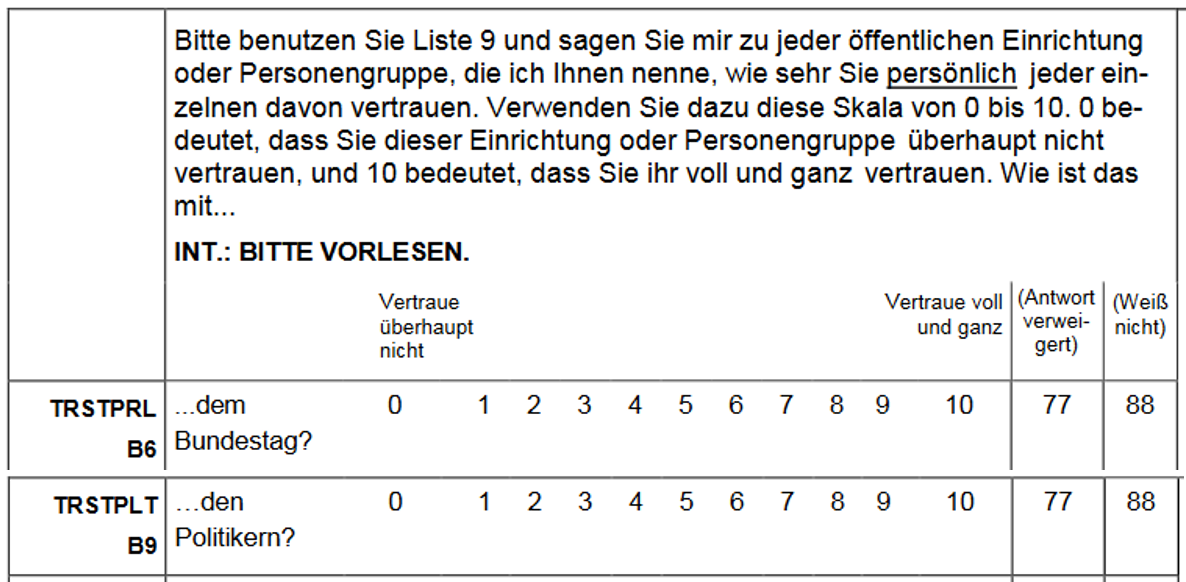
\includegraphics[width=\textwidth]{pics/s5-1.png}
	\end{figure}
\end{center}

\end{frame}

\begin{frame}[t]{Quick-Feedback}
4 Kurze Fragen: 

\begin{itemize}
	\item Für mich ist das Lerntempo in Ordnung.
	\item Für mich ist Lernfortschritt erkennbar.
	\item Der Wechsel von Plenum und Kleingruppen ist bisher gut.
	\item Freies Feedback
\end{itemize}

Bitte am Ende der Umfrage auf Senden klicken!

\end{frame}

\renewcommand*{\bibfont}{\scriptsize}

\begin{frame}[allowframebreaks]{Literatur}
	\nocite{*}
	\printbibliography[heading = none]
\end{frame}

\section{Mittagspause! \\ Wir treffen uns um 12:30 Uhr wieder.}

\end{document}